
\documentclass{beamer}
\usepackage[utf8]{inputenc}
\usepackage[spanish]{babel}
\usetheme{Madrid}
\title{Sesión 6: Árboles de Decisión (CART), Poda, ROC y AUC}
\author{Oscar Leonardo Rincón León }
\date{}

\begin{document}

\frame{\titlepage}

\begin{frame}{Objetivo}
Aplicar árboles de decisión e interpretar reglas. Evaluar rendimiento con métricas visuales como la curva ROC y el AUC.
\end{frame}

\begin{frame}{¿Qué es un árbol de decisión?}
\begin{itemize}
    \item Modelo predictivo basado en reglas jerárquicas.
    \item Representa decisiones con condiciones anidadas.
    \item CART: algoritmo clásico que construye árboles binarios.
\end{itemize}
\end{frame}

\begin{frame}{Características de CART}
\begin{itemize}
    \item Árboles binarios: cada nodo tiene dos ramas.
    \item Clasificación: impureza de Gini o entropía.
    \item Regresión: minimiza el error cuadrático medio (MSE).
    \item Salida: reglas tipo “si... entonces...”.
\end{itemize}
\end{frame}

\begin{frame}{Terminología básica}
\begin{itemize}
    \item Nodo raíz: nodo inicial con todos los datos.
    \item Nodo interno: evalúa una condición de división.
    \item Hoja: nodo terminal con una clase o valor.
    \item Profundidad: número de niveles del árbol.
\end{itemize}
\end{frame}

\begin{frame}{Sobreajuste y profundidad}
\begin{itemize}
    \item Árboles profundos capturan ruido del entrenamiento.
    \item Pérdida de generalización: sobreajuste.
    \item Árboles poco profundos: subajuste.
    \item Balance necesario mediante validación.
\end{itemize}
\end{frame}

\begin{frame}{¿Qué es la poda?}
\begin{itemize}
    \item Reduce complejidad del árbol para evitar sobreajuste.
    \item Mejora la generalización.
\end{itemize}
\textbf{Tipos de poda:}
\begin{itemize}
    \item Poda previa: limitar profundidad o tamaño mínimo.
    \item Poda posterior: eliminar nodos irrelevantes tras el entrenamiento.
\end{itemize}
\end{frame}

\begin{frame}{Ejemplo visual de poda}
\centering
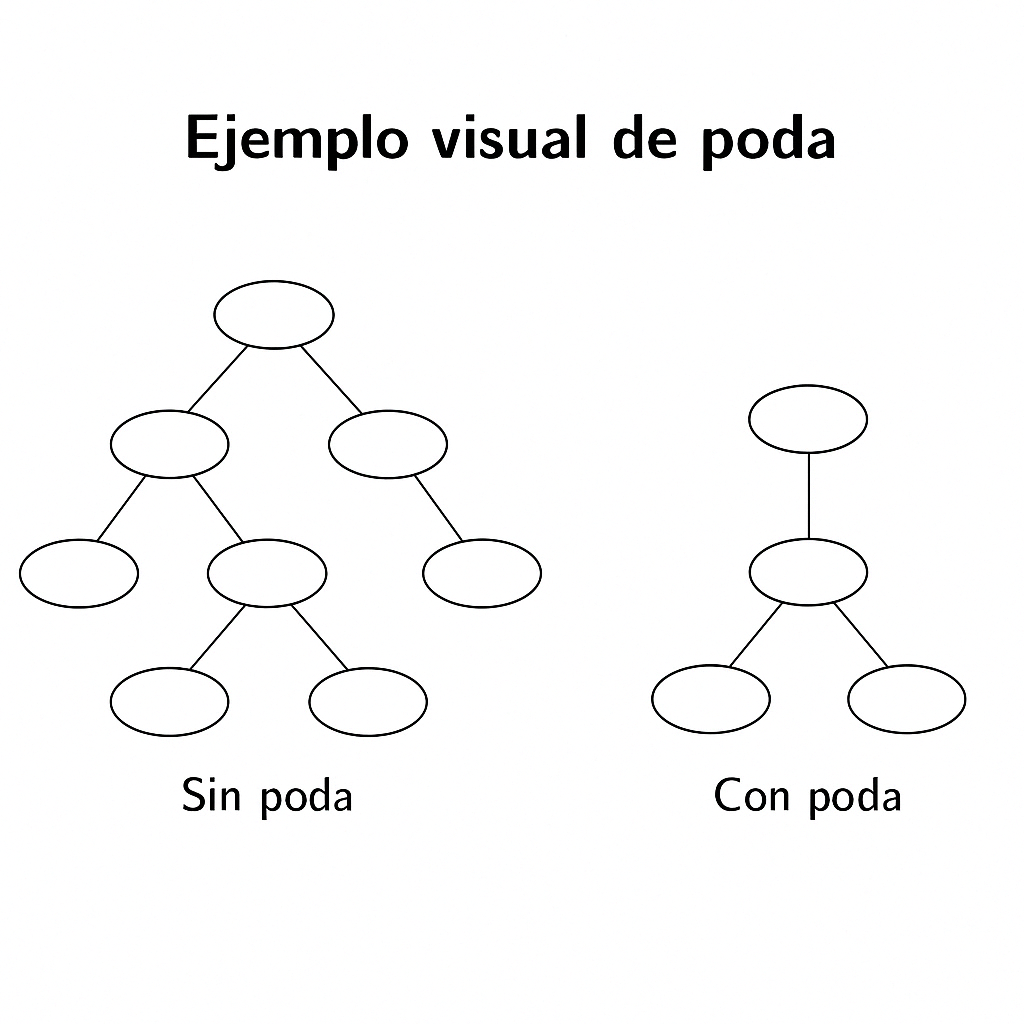
\includegraphics[width=0.4\textwidth]{example-tree.png}
\end{frame}

\begin{frame}{Evaluación del modelo}
\begin{itemize}
    \item Matriz de confusión.
    \item Precisión, Recall, F1.
    \item Curva ROC y AUC.
\end{itemize}
\end{frame}

\begin{frame}{Curva ROC}
\begin{itemize}
    \item ROC: compara sensibilidad (TPR) vs tasa de falsos positivos (FPR).
    \item Muestra el rendimiento según distintos umbrales.
    \item Ideal: curva cercana al vértice superior izquierdo.
\end{itemize}
\end{frame}

\begin{frame}{AUC: Área bajo la curva}
\begin{itemize}
    \item Mide capacidad de discriminación.
    \item AUC = 1: modelo perfecto. AUC = 0.5: aleatorio.
    \item Permite comparar modelos sin fijar umbral.
\end{itemize}
\end{frame}

\begin{frame}{Aplicaciones prácticas}
\begin{itemize}
    \item Clasificación de hogares vulnerables.
    \item Segmentación por riesgo financiero.
    \item Justificación de reglas ante actores sociales.
\end{itemize}
\end{frame}

\begin{frame}{Actividad práctica}
\begin{itemize}
    \item Entrenar árbol con y sin poda.
    \item Visualizar árbol y extraer reglas.
    \item Comparar desempeño con matriz y AUC.
\end{itemize}
\end{frame}

\begin{frame}{Discusión final}
\begin{itemize}
    \item ¿Qué variables fueron más relevantes?
    \item Interpretabilidad vs precisión.
    \item ¿Es útil un árbol para justificar decisiones?
\end{itemize}
\end{frame}

\end{document}
